The purpose of this report is to simulate the end-to-end transmission of a data message using convolutional codes. Figure \ref{fig:simulationOverview} shows the logical setup of the simulation.

\begin{figure} [h]
\usetikzlibrary{shapes,arrows}

\tikzstyle{block} = [draw, rectangle, minimum height=3em, minimum width=6em]
\tikzstyle{input} = [coordinate]
\tikzstyle{output} = [coordinate]

\centering
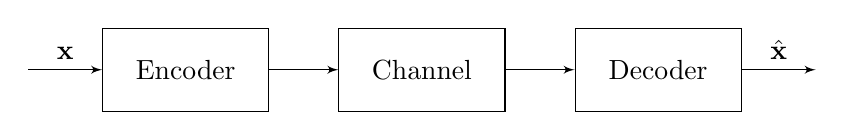
\begin{tikzpicture}[auto, node distance=2cm,>=latex']
\centering

    % We start by placing the blocks
    \node [input, name=input] {};    
    \node [block, right of=input] (encoder) {Encoder};
    \node [block, right of=encoder, node distance=3cm] (channel){Channel};
    \node [block, right of=channel, node distance=3cm] (decoder){Decoder};
    \node [output, right of=decoder] (output) {}; 
    
    
    \draw [->] (encoder) -- node[name=u] {} (channel);
    \draw [->] (channel) -- node[name=v] {} (decoder);
    \draw [draw,->] (input) -- node {$\textbf{x}$} (encoder);
    \draw [->] (decoder) -- node [name=y] {$\hat{\textbf{x}}$}(output);

\end{tikzpicture}
\caption{Simulation overview \label{fig:simulationOverview}}
\end{figure}

A message of an arbitrary length is sent over a noisy channel. The 2 types of channels considered in this simulation scenario are:
\begin{itemize}
   \item BSC - binary symmetric channel - where random errors at random positions occur. The typical representation of a binary symmetric channel is shown in figure \ref{fig:bscChannel}
   \item Burst error channel - where errors appear one after another - forming a larger burst error
\end{itemize}

\begin{figure} [h]
\centering
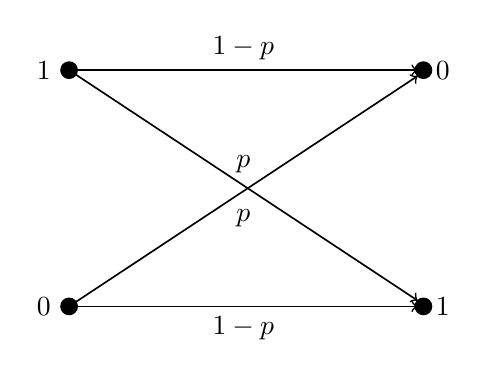
\begin{tikzpicture}
\centering
\filldraw (0,0) circle (3pt);
\filldraw (0,3) circle (3pt);
\filldraw (4.5,0) circle (3pt);
\filldraw (4.5,3) circle (3pt);
\draw[->,line width=0.6pt] (0,3) node[left=3pt] {$1$} -- node[above=1pt] {$p$} (4.425,0.075);
\draw[->,line width=0.6pt] (0,0) node[left=3pt] {$0$} -- node[below=3pt] {$p$} (4.425,2.925);
\draw[->,line width=0.6pt] (0,0) -- node[below] {$1-p$} (4.425,0.00)  node[right=3pt] {$1$};
\draw[->,line width=0.6pt] (0,3) -- node[above] {$1-p$} (4.425,3) node[right=3pt] {$0$};
\end{tikzpicture}
\caption{Binary Symmetric Channel\label{fig:bscChannel}}
\end{figure}

The purpose of the simulation is to determine the effects introduced by modifying the different parameters of the convolutional code, namely the constraint length and the code rate while keeping the free distance constant. In order to achieve the best performance a trade-off analysis on the parameters needs to be performed.

The simulation is constructed using Matlab. Section \ref{sec:methodSection} presents the approach we used in order to systematically determine the result variations and the subsequent sections present the results. In section \ref{sec:conclusionSection} we summarize the findings and provide our interpretation.


